
\documentclass[10pt,a4paper]{article}
\usepackage[margin=0.72in,top=0.6in,bottom=0.6in]{geometry}
\usepackage{graphicx,booktabs,enumitem,xcolor,amsmath}
\usepackage[hidelinks]{hyperref}
\usepackage{parskip}
\pagestyle{empty}
\setlist{itemsep=1.5pt,topsep=2pt,leftmargin=1.2em}
\definecolor{ink2}{HTML}{52514E}
\newcommand{\hd}[1]{\par\vspace{3pt}{\large\bfseries #1}\par\vspace{-2pt}}
\begin{document}

{\LARGE\bfseries How much does each assumption matter?}\\[2pt]
{\large A sensitivity exercise on the AICD/Mandala estimate of Commonwealth compliance costs}\\[2pt]
{\small\color{ink2}Laural Alex Jacob \;|\; October 2026 \;|\; An independent exercise using published figures. Not affiliated with Mandala or the AICD. Model and code: github.com/laj07/aicd-sensitivity}

\hd{Why I looked at this}
I read Mandala's report for the AICD (\emph{\$160 billion and counting}, Nov 2025) and wanted to understand how the headline is put together. I build and test quantitative models, and the best way I know to understand an estimate is to rebuild it and see which inputs move it. This note records what I learned. It uses only the report's published figures, and I would welcome corrections where I have misread the method.

\hd{What I did}
I rebuilt the three methods from the inputs printed on pp.\ 27, 39 and 40, in Excel with live formulas and in Python, and cross-checked the result in R; tests confirm they agree. I then moved each input by 20\%, re-ran the model under named alternative choices, ran a Monte Carlo with stated ranges, and backed the uncertainty in the investment regression out of its p-value. Every input is recorded with its page number in \texttt{data/inputs.csv} so it can be checked against the slides.

\hd{What I found}
The order of magnitude was stable across everything I tried: the lowest case I computed is still \$123B a year.
\begin{itemize}
\item \textbf{The headline rebuilds closely.} The report's formulas on its printed inputs give \$190B, \$152B and \$133B (printed: \$190B, \$150B and about \$130B), averaging \$159B (printed: \$159B). Method 3 matches once the 96 million hours the report excludes are removed.
\item \textbf{Methods 1 and 2 build on the same 2013 estimate} of \$65B, as the report describes, so 72\% of the headline moves with that one figure. Method 3 is built up from 2024 inputs and is the lowest of the three.
\item \textbf{Two inputs carry more weight than the others.} The +35\% complexity multiplier averages six metrics, and the largest, notional amendments (+141\%), is 67\% of their combined change; without it Method 1 is \$161B and the headline \$149B. In Method 3, ordinary staff time is 64\% of the line items, at 87 hours a worker a year; at 60 hours the headline is \$147B.
\item \textbf{Other reasonable choices} move the headline between \$139B and \$156B one at a time, and to \$123B with four together. Letting the main drivers vary 25\% either way gives an 80\% range of \$143B to \$174B.
\item \textbf{A 25\% cut is worth \$31B to \$48B} depending on method and choices, against \$40B at the headline. A percentage target is less sensitive to these choices than a dollar figure.
\end{itemize}

\begin{center}
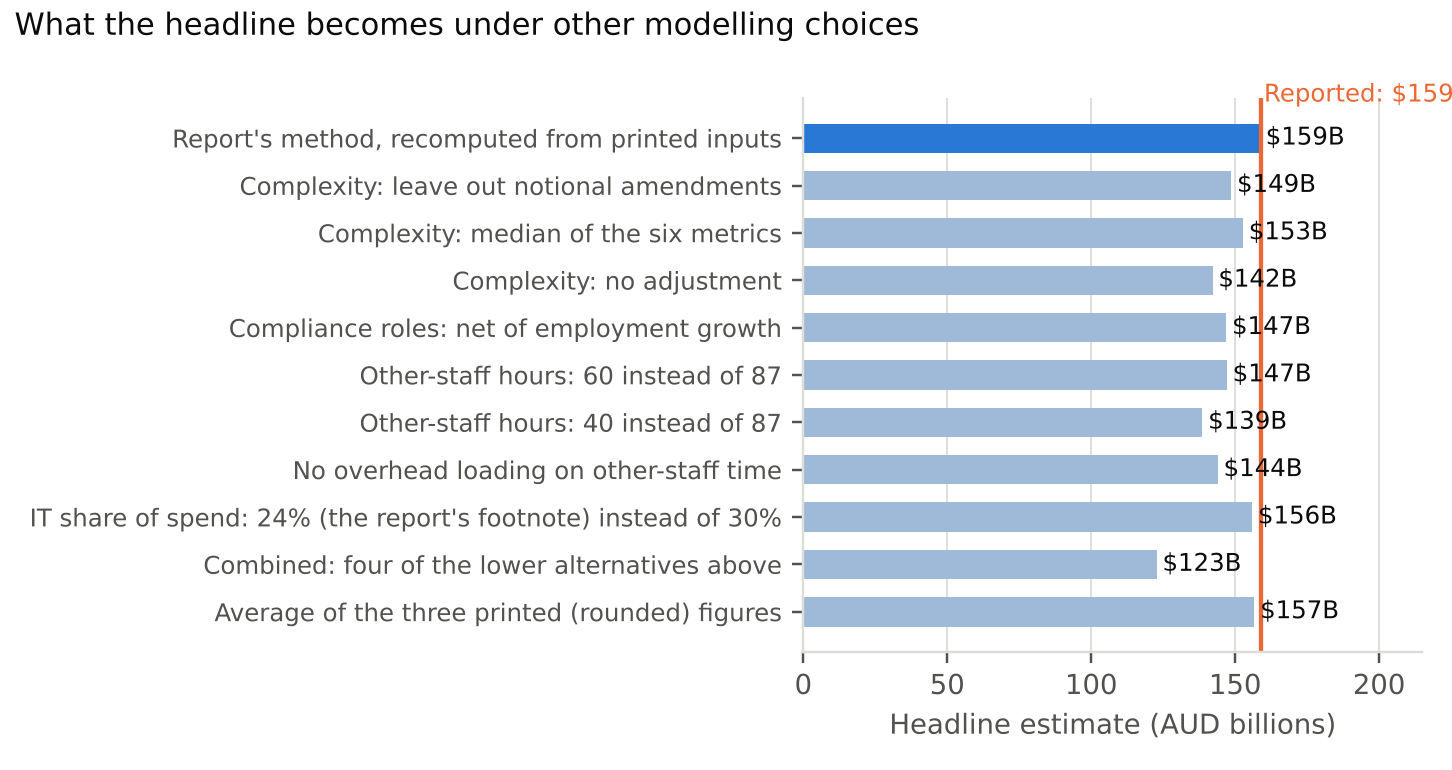
\includegraphics[width=0.78\linewidth]{../outputs/figs/fig3_scenarios.png}
\end{center}

\hd{Questions this raised}
These are for someone who knows the method better than I do.
\begin{enumerate}
\item \textbf{The IT share.} The IT line uses 30\% of \$135B, giving \$41B, while the source column describes a 24\% share (the average of 30\% from stakeholder insights and 17\% from the US banking survey). At 24\% Method 3 is \$125B and the headline \$156B. I may be misreading the source column, so I would value knowing which share is intended.
\item \textbf{The 87 hours.} It comes from a small-business survey (9.3 hours per business per week, shared across small-business employees) and is applied to all 14.3 million workers. Given how much of Method 3 rests on it, I was curious how the team thinks about its range.
\item \textbf{The investment result.} The coefficient of $-22.4$ with $p=0.09$ implies a standard error of about 13.2 and a 95\% interval from $-48$ to $+3.5$. At the ends of that interval, foregone investment ranges from a loss of \$22.4B to a gain of \$1.6B, against the printed \$10.4B. The report describes the result as marginal, which fits; I wondered how it is weighed alongside the direct cost estimate.
\item \textbf{Costs and benefits.} The estimate counts costs. I was curious how the team thinks about pairing it with the benefits side, such as the protections that followed the Royal Commissions.
\end{enumerate}

\begin{center}
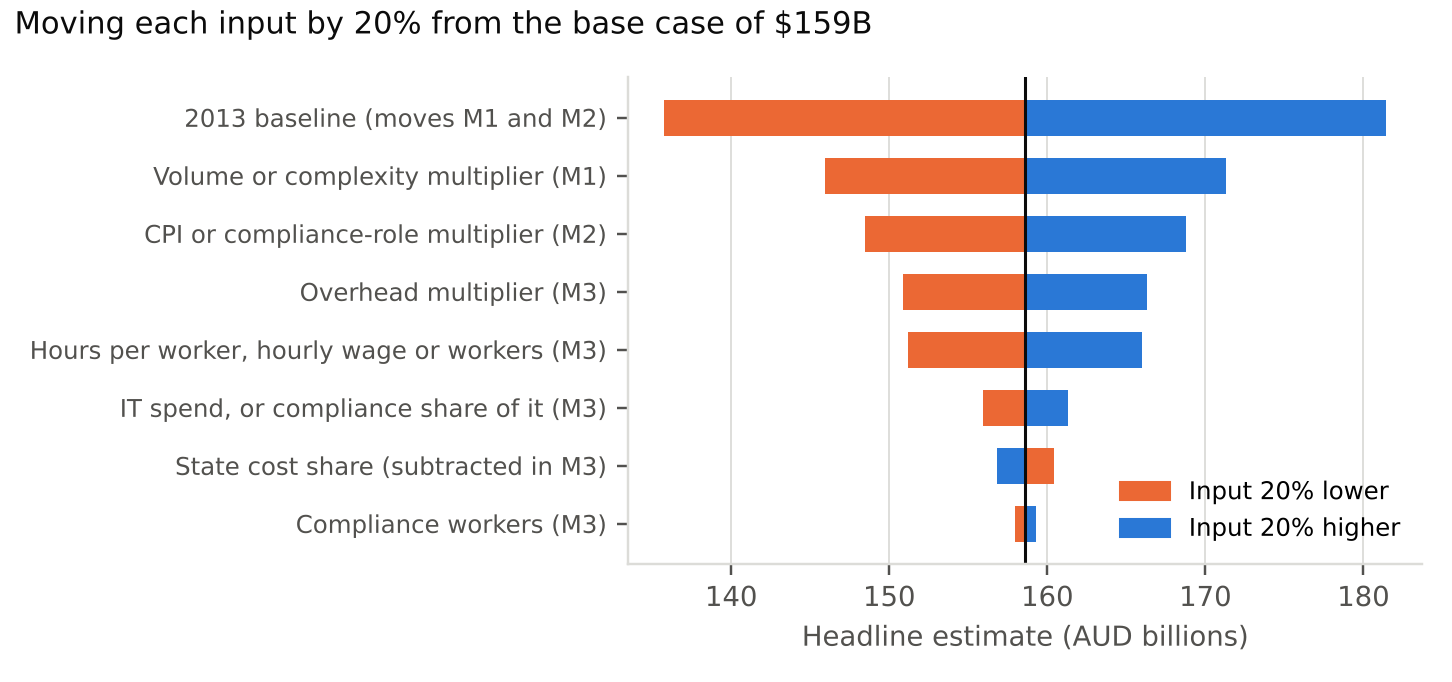
\includegraphics[width=0.78\linewidth]{../outputs/figs/fig2_tornado.png}
\end{center}

\hd{Limits}
I tested the departures the arithmetic allows, not upward cases such as state and local regulation, which the report leaves out. Hours of 60 and 40 and no overhead on staff time are my own choices, not figures from the report; the 24\% IT share is the one in the report's own source column. The employment-growth adjustment uses the report's 30\% for 2010--24 and should be checked against ABS data for 2013--24. The regression uses non-public data and I could not replicate it; the interval is backed out of the printed p-value.

\hd{A related question from my own work}
CallFlag, a tool I built that was a finalist in the Forward: AI in Business Hackathon, flags National Credit Code obligations during bank hardship calls, where a wrong flag starts a 21-day legal clock. It faces a version of the same trade-off at call level: flag only when the evidence passes $c_{\mathrm{fp}}/(c_{\mathrm{fp}}+c_{\mathrm{miss}})$, where $c_{\mathrm{fp}}$ is the cost of a false flag and $c_{\mathrm{miss}}$ the cost of a miss. Your report made me curious how that trade-off looks at the scale of the economy.

\end{document}
